% Chapter Template

\chapter{Laminated Composite Material Optimization by New Genetic Algorithm Model} % Main chapter title

\label{Chapter4} % Change X to a consecutive number; for referencing this chapter elsewhere, use \ref{ChapterX}


\section{Case1: Maximum Strength Optimization}
\begin{table*}[ht]
\caption{Comparison of the carbon/epoxy, graphite/epoxy, and glass/epoxy properties}
\centering
\begin{adjustbox}{width=1\textwidth}
\label{tab:mat}
\begin{tabular}{cccccc}
\toprule
Property								   & Symbol				  & Unit  &  Carbon/Epoxy&  Graphite/Epoxy  &  Glass/Epoxy   \\
\midrule
Longitudinal elastic modulus			   & $E_1$				  & GPa   &  116.6       &  181             &  38.6           \\
Traverse elastic modulus				   & $E_2$				  & GPa   &  7.67        &  10.3            &  8.27           \\
Major Poisson's ratio					   & $v_{12}$			  &       &  0.27        &  0.28            &  0.26           \\
Shear modulus							   & $G_{12}$			  & GPa   &  4.17        &  7.17            &  4.14           \\
Ultimate longitudinal tensile strength     & $(\sigma_1^T)_{ult}$ & MP    &  2062        &  1500            &  1062            \\
Ultimate longitudinal compressive strength & $(\sigma_1^C)_{ult}$ & MP    &  1701        &  1500            &  610             \\
Ultimate transverse tensile strength       & $(\sigma_2^T)_{ult}$ & MPa   &  70          &  40              &  31              \\
Ultimate transverse compressive strength   & $(\sigma_2^C)_{ult}$ & MPa   &  240         &  246             &  118              \\
Ultimate in-plane shear strength           & $(\tau_{12})_{ult}$  & MPa   &  105         &  68              &  72               \\
Density                                    & $\rho$               & $g/cm^3$ &  1.605    &  1.590           &  1.903               \\
Cost                                       &                      &       &  8           &  2.5             &  1               \\
\bottomrule
\end{tabular}
\end{adjustbox}
\end{table*}

\begin{table*}[!htb]
\caption{The optimum lay-ups for the loading $N_x=1e6$ N}
\centering
\begin{adjustbox}{width=1\textwidth}
\begin{tabular}{c|cc|cc}
	\toprule
	Cross Ply $[0_M/90_N]$         & \multicolumn{2}{c}{Previous Research} & \multicolumn{2}{c}{Current Research} \\
	\midrule																								  
	 Material       &  Glass-Epoxy & Graphite-Epoxy  & Glass-Epoxy & Graphite-Epoxy      \\ 
	      M         &  68          &    17           &  78		    &  18             \\
	      N         &  72          &    18           &  28		    &  8              \\
no. of lamina(n)    &  140         &    35           &  106	    &  26                     \\
         SR         &  2.01        &    2.10         &  2.03	    &  2.16            \\
     weight         &  9.10        &    1.84         &  6.89	    &  102.5           \\
	\bottomrule
\end{tabular}
\end{adjustbox}
\label{tab:comparsion}
\end{table*}


\subsection{Methodology}

\subsection{Result and Discussion}

\section{Case2: Minimum Thickness Optimization}
In this case, the mentioned NGAM in chapter three is taken to minimize thickness(or
weight) of mid-plane symmetric composite laminate subject to in-plane loading.
Fiber orientation and ply thickness are chosen as design variables, the proposed
Tsai-wu and the maximum stress criteria are employed to determine whether
load bearing capacity is exceeded or not.

\subsection{Methodology}

The optimization problem can be formulated as searching the optimal stacking
sequence of composite laminate. There are two design variables in this problem,
the angles in the laminate, and the number of layers that each fiber orientation
has. The final objective function is given as

\begin{equation}
	\begin{split}
    	F  &= 2t_0 \sum_{k=1}^n n_k  \textstyle{,}\\
    	   &SF_{MS} \geq 1 \textstyle{,} \\
    	   &SF_{TW} \geq 1 \textstyle{.}
	\end{split} 
\end{equation}

The first term represents the total thickness of the composite laminates, $t_0$
is the ply thickness; $n_k$ is the number of plies in the kth lamina, in which
the fiber orientation is $\theta_k$. The constraints here are two safety
factors should not less than 1, which means  $SF_{MS} \geq 1$, and $SF_{TW} \geq
1$, respectively.

\subsection{Encoding}
Due to the simplicity and efficiency of float representation, this encoding
method is implemented to represent a possible solution. As shown in Figure \ref{GA:operator}
 (a), these two chromsomes represent a $[+8_{7}/-9_{2}]_s$
carbon T300/5308 laminated composite, and $[+19_{4}/-36_{6}]_s$, respectively.
Becasue the laminate adopted in this paper is symmetric to its mid-plane, so
only half needs to be encoded.

\afterpage{

\begin{figure}
\setlength{\fboxsep}{0pt}%
\setlength{\fboxrule}{0pt}%
\begin{center}
\resizebox{.95\linewidth}{!}{
		\begin{tikzpicture}
		\tikzstyle{rec} = [rectangle, minimum width=0.8cm,minimum height=0.6cm, text
		centered, draw=black]
			\node (gene11) [rec] {+7};
			\node (gene2) [rec] at ($(gene11.east)+(0.4cm,0)$)  {+7};
			\node (gene3) [rec] at ($(gene2.east)+(0.4cm,0)$)  {+7};
			\node (gene4) [rec] at ($(gene3.east)+(0.4cm,0)$)  {+7};
			\node (gene5) [rec] at ($(gene4.east)+(0.4cm,0)$)  {+7};
			\node (gene6) [rec] at ($(gene5.east)+(0.4cm,0)$)  {+7};
			\node (gene7) [rec] at ($(gene6.east)+(0.4cm,0)$)  {+7};
			\node (gene8) [rec] at ($(gene7.east)+(0.4cm,0)$)  {+7};
			\node (gene9) [rec] at ($(gene8.east)+(0.4cm,0)$)  {-9};
			\node (last) [rec] at ($(gene9.east)+(0.4cm,0)$)  {-9};
			\node[text width=1cm] at ($(gene11.west)+(-0.3cm,0)$) {$P_1$:};
			\node (gene1) [rec] at ($(gene11.east)+(-0.4cm,-0.8cm)$) {+19};
			\node (gene2) [rec] at ($(gene1.east)+(0.4cm,0)$)  {+19};
			\node (gene3) [rec] at ($(gene2.east)+(0.4cm,0)$)  {+19};
			\node (gene4) [rec] at ($(gene3.east)+(0.4cm,0)$)  {+19};
			\node (gene5) [rec] at ($(gene4.east)+(0.4cm,0)$)  {-36};
			\node (gene6) [rec] at ($(gene5.east)+(0.4cm,0)$)  {-36};
			\node (gene7) [rec] at ($(gene6.east)+(0.4cm,0)$)  {-36};
			\node (gene8) [rec] at ($(gene7.east)+(0.4cm,0)$)  {-36};
			\node (gene9) [rec] at ($(gene8.east)+(0.4cm,0)$)  {-36};
			\node (gene10) [rec] at ($(gene9.east)+(0.4cm,0)$)  {-36};
			\node[text width=1cm] at ($(gene1.west)+(-0.3cm,0)$) {$P_2$:};
			\draw[-,white] ($(gene10.north)$)-- ++(0,-1.5cm);
			\node (label1) at ($(gene5.south)+(0cm,-0.5cm)$) {(a): Parents $P_1$ and $P_2$};
		\end{tikzpicture}
}

% offspring
\resizebox{.95\linewidth}{!}{
		\begin{tikzpicture}
			\tikzstyle{rec} = [rectangle, minimum width=0.8cm,minimum height=0.6cm, text
			centered, draw=black]
			\node (gene11) [rec] {+13};
			\node (gene2) [rec] at ($(gene11.east)+(0.4cm,0)$)  {+13};
			\node (gene3) [rec] at ($(gene2.east)+(0.4cm,0)$)  {+13};
			\node (gene4) [rec] at ($(gene3.east)+(0.4cm,0)$)  {+13};
			\node (gene5) [rec] at ($(gene4.east)+(0.4cm,0)$)  {+13};
			\node (gene6) [rec] at ($(gene5.east)+(0.4cm,0)$)  {+13};
			\node (gene7) [rec] at ($(gene6.east)+(0.4cm,0)$)  {-27};
			\node (gene8) [rec] at ($(gene7.east)+(0.4cm,0)$)  {-27};
			\node (gene9) [rec] at ($(gene8.east)+(0.4cm,0)$)  {-27};
			\node (last) [rec] at ($(gene9.east)+(0.4cm,0)$)  {-27};
			\node[text width=1cm] at ($(gene11.west)+(-0.3cm,0)$) {$O_1$:};
			\node (gene1) [rec] at ($(gene11.east)+(-0.4cm,-0.8cm)$) {+22};
			\node (gene2) [rec] at ($(gene1.east)+(0.4cm,0)$)  {+22};
			\node (gene3) [rec] at ($(gene2.east)+(0.4cm,0)$)  {+22};
			\node (gene4) [rec] at ($(gene3.east)+(0.4cm,0)$)  {+22};
			\node (gene5) [rec] at ($(gene4.east)+(0.4cm,0)$)  {+22};
			\node (gene6) [rec] at ($(gene5.east)+(0.4cm,0)$)  {+22};
			\node (gene7) [rec] at ($(gene6.east)+(0.4cm,0)$)  {+22};
			\node (gene8) [rec] at ($(gene7.east)+(0.4cm,0)$)  {+5};
			\node (gene9) [rec] at ($(gene8.east)+(0.4cm,0)$)  {+5};
			\node (gene10) [rec] at ($(gene9.east)+(0.4cm,0)$)  {+5};
			\node[text width=1cm] at ($(gene1.west)+(-0.3cm,0)$) {$O_2$:};
			\draw[-,white] ($(gene10.north)$)-- ++(0,-1.5cm);
			\node (label1) at ($(gene5.south)+(0cm,-0.5cm)$) {(b): Offspring $O_1$ and $O_2$};
		\end{tikzpicture}
}

%mutation
\resizebox{.95\linewidth}{!}{
	\begin{tikzpicture}
	\tikzstyle{rec} = [rectangle, minimum width=0.8cm,minimum height=0.6cm, text
	centered, draw=black]
		\tikzstyle{rec} = [rectangle, minimum width=0.8cm,minimum height=0.6cm, text
		centered, draw=black]
		%\draw[help lines](-3,-3) grid (4,4);
		\node (gene11) [rec] {+13};
		\node (gene2) [rec] at ($(gene11.east)+(0.4cm,0)$)  {+13};
		\node (gene3) [rec] at ($(gene2.east)+(0.4cm,0)$)  {+13};
		\node (gene4) [rec] at ($(gene3.east)+(0.4cm,0)$)  {$\cdots$};
		\node (gene5) [rec] at ($(gene4.east)+(0.4cm,0)$)  {+13};
		\node (gene6) [rec] at ($(gene5.east)+(0.4cm,0)$)  {+13};
		\node (gene7) [rec] at ($(gene6.east)+(0.4cm,0)$)  {-27};
		\node (gene8) [rec] at ($(gene7.east)+(0.4cm,0)$)  {$\cdots$};
		\node (gene9) [rec] at ($(gene8.east)+(0.4cm,0)$)  {-27};
		\node (last) [rec] at ($(gene9.east)+(0.4cm,0)$)  {-27};
		\draw[<->,thick] (gene11.south) .. controls +(1.8,-0.4) .. (gene6.south)
			node[pos=0.5] {11} ;
		\draw[<->,thick] (gene7.south) .. controls +(1.3,-0.4) .. (last.south)
			node[pos=0.5] {7};
		\node[text width=1cm] at ($(gene11.west)+(-0.3cm,0)$) {$O_1$:};

		\node (label1) at ($(gene5.south)+(0cm,-0.8cm)$) {(c): Offspring $O_1$ after
			lenght mutation};

		\node (gene1) [rec] at ($(gene11.east)+(-0.4cm,-1.8cm)$) {+12};
		\node (gene2) [rec] at ($(gene1.east)+(0.4cm,0)$)  {+12};
		\node (gene3) [rec] at ($(gene2.east)+(0.4cm,0)$)  {+12};
		\node (gene4) [rec] at ($(gene3.east)+(0.4cm,0)$)  {$\cdots$};
		\node (gene5) [rec] at ($(gene4.east)+(0.4cm,0)$)  {+12};
		\node (gene6) [rec] at ($(gene5.east)+(0.4cm,0)$)  {+12};
		\node (gene7) [rec] at ($(gene6.east)+(0.4cm,0)$)  {-26};
		\node (gene8) [rec] at ($(gene7.east)+(0.4cm,0)$)  {$\cdots$};
		\node (gene9) [rec] at ($(gene8.east)+(0.4cm,0)$)  {-26};
		\node (last) [rec] at ($(gene9.east)+(0.4cm,0)$)  {-26};
		\node[text width=1cm] at ($(gene11.west)+(-0.3cm,0)$) {$O_1$:};
		\draw[-,white] ($(gene10.north)$)-- ++(0,-1.5cm);
		\node (label1) at ($(gene5.south)+(0cm,-0.5cm)$) {(b): Offspring $O_1$ 
			 after angle mutation};
	\end{tikzpicture}
}
\end{center}
\caption{GA Operators\label{GA:operator}}
\end{figure}

\clearpage
}

\subsection{Selection}
The purpose of the selection operator is to chose mating pool to produce
alternative solutions of better fitness. Traditional methods of selecting
strategies only take the fitness of individuals into acount, however, due to 
the existance of constraint, various selection schemes are implemented to
selecet the mating set. Based on different selection schemes, the parents of
next generation can be divided into  three groups: proper groups, active groups,
and potential groups according to different selecting methods. 

Proper parents mean in which individual fullfils the constraints, which are
chosen by the individual's fitnees, individuals with better fitness are more
likely to be chosen if they fit the constraint; active groups means that
individual is supposed to be always exist in the parents during the GA, which
are selected by fitness, ignoring the constraint; The individuals from active
group may not correspond to feasible solutions, but their existance enriches the
variety of the gene clips.  Potential groups means that they are likely to turn
into proper individual after a couple of generations, and potential individuals
are chosen by constraint function, the more the individual fulfils the
constraint, the more possiblity it will be selected.

\subsection{Crossover}
The crossover operator happens among these three groups. the child of two proper
groups are more likely to be a proper individual which can be used to obtain a
alternative feasible solution. the child of an active individual and a potential
individual can significantly change the gene of active individual's chromsome,
which makes the individual evolve toward a new direction. The offspring of two
active individuals are more likely to be an active individual, which can maitain
the active group.  The figure.\ref{GA:operator} (b) shows two children $O_1$
and $O_2$ from two parents $P_1$ and $P_2$, each angle $C_a$ and it's length 
$C_l$ of a child are obtained by the following formula

\begin{align} 
	\begin{cases}
	C_a &= (P1_a + P2_a)/2 \\
	C_l &= (P1_l + P2_l)/2 
\end{cases} \textstyle{.}
\end{align}

\subsection{Mutation}
A mutation direction is imposed on the mutation operator which to make sure the
individual evolving toward the right direction. The mutation direction, denoted
by $md$, is a n dimensional vector corresonding to the number of constraints, it
is decided by the constraint thresholds $CT_i$ and the current individual's
constraint value, denoted as $CV_i$,  The mutation vector can be obtained by the
following formula

\resizebox{.9\linewidth}{!}{
	$\text{md} = [CT_1, \cdots, CT_{n-1}, CT_n] -  [CV_0, \cdots, CV_{n-1}, CV_n]$
}

During the operator, the mutation procedure is consist of two phases: the length
mutation of the chromsome, and the angle mutation of the chromsome.  Becasue the
chromsome's length is positive correlated with the individual's fitness, the
coefficient of length mutation denoted by $C_l$, if $\sum_{i=1}^{N}{CT_i}$ great
than $\sum_{i=1}^{N}{CV_i}$ , the mutation length is restricted to the range
$[0,(C_l \sum_{i=1}^{N}{(CT_i-CV_i)})/N]$, which means increase the chromsome's
length;Assuming a $[+13_6/-27_4]_s$ T300/5308 carbon/epoxy composite
laminate under the loading $N_{x} = N_{y} = 10$ MPa m, it's property as shown
in table \ref{tab:T300/5308}. According to CLT and
failure theory, the two safety factors $SF_{MS}$ and $SF_{TW}$ are  0.0539, and
0.0540, respectively. So the mutation vector and is $[0.9461,0.9460]$, assuming
the length mutation coefficient is 20, so the mutation range is from 0 to 18. A
random number is generated from the range $[0, 18]$, supposing the outcome is
13, then a length generator is used to a list, the it's sum is 13, suppose the
list is [5, 8], the laminate after mutation is $[13_{11}/-27_{12}]_s$.

If the $\sum_{i=1}^{N}{CT_i}$ less than $\sum_{i=1}^{N}{CV_i}$, the
mutation length is restricted to the range $([\sum_{i=1}^{N}{CT_i-CV_i})/N,0]$,
which means the individual's fitness exceeds the threshold value, and decrease
the chromsome's length.  Assuming a $[+33_{35}/-29_{26}]_s$ T300/5308 laminate
is under loading $N_{x}=10$ MPa, and $N_{y}=5$ MPa, then, it's $SF_{MS}$
constraint and $SF_{TW}$ values are  1.0912, 1.0747, respectively.
because the length mutation is 20, so the mutation range is from -2 to 0. This
would decrease the chromsome's length. 

\begin{align}
	\text{LM} = 
	\begin{cases}
		\resizebox{.35\textwidth}{!}{$[0,(C_l \sum_{i=1}^{N}{(CT_i-CV_i)})/N], \text{ if }  \sum_{i=1}^{N}{CT_i} > 
		\sum_{i=1}^{N}{CV_i}$}\\
		\resizebox{.35\textwidth}{!}{$[(C_l \sum_{i=1}^{N}{(CT_i-CV_i)})/N,0], \text{ if }  \sum_{i=1}^{N}{CT_i} < 
		\sum_{i=1}^{N}{CV_i}$}\\
	\end{cases} 
\end{align}

The relationship between the angles in the composite laminate and the
chromsome's fitness is unclear, so the mutation direction of chromsome's angle
is random. The coefficient angle mutation is $C_a$, the angle mutation range is
$[0,C_a \sum_{i=1}^{N}{(|CT_i-CV_i|)}]$ or $[C_a
\sum_{i=1}^{N}{(-|CT_i-CV_i|)},0]$. It is can be written as

\begin{align}
	\text{P(AM)} =  
	\begin{cases}
		0.5, \text{ AM = }[0,C_a \sum_{i=1}^{N}{(|CT_i-CV_i|)}] \\ 
	    0.5, \text{ AM = }[C_a \sum_{i=1}^{N}{(-|CT_i-CV_i|)},0]
	\end{cases} \textstyle{.}
\end{align}


\begin{table*}
	\normalsize
\caption{The optimum lay-ups using two distinct fiber angles under various biaxial loading cases}
\label{tab:two_distinct_angle}
\centering
\resizebox{13cm}{!}{
\begin{tabular}{clccc}
	\toprule
	\textbf{Loading} $N_{x}/N_{y}/N_{xy}$ \textbf{(MPa m)}   &
	\makecell{\textbf{Optimum lay-up } \\ \textbf{sequences}  }                        &
	\textbf{Laminate thickness} &  \makecell{\textbf{Safety factor } \\
	\textbf{for Tsai-wu}}  &
	\makecell{\textbf{Safety factor } \\ \textbf{for  maximum stress}}
	 \\
	\midrule
	10/5/0                                         &  $[33_{29}/\text{-}39_{25}/\bar{\text{-}39}]_s$            &     109               &  1.0074      &  1.0246  \\
	20/5/0                                         &  $[33_{22}/\text{-}31_{24}]_s$                             &     92               &  1.0055       &  1.2065    \\
	40/5/0                                         &  $[29_{18}/\text{-}21_{23}/\bar{\text{-}21}]_s$            &     83               &  1.0034       &  1.7350   \\
	80/5/0                                         &  $[\text{-}20_{27}/21_{25}/\bar{25}]_s$                    &     105               &  1.0029      &  1.2063    \\
	120/5/0                                         &  $[\text{-}18_{34}/17_{36}]_s$                            &     140               &  1.0000      &  1.0898    \\
	\bottomrule
\end{tabular}
}
\end{table*}







\subsection{Result and Discussion}
In present study, the T300/5308 graphite/epoxy material is used in the
lay-up sequence optimization, and it's properties as shown in
table.\ref{tab:T300/5308}. Two constraints are imposed on the composite
laminates which are the safety factor $SF_{MS}$ , and safety factor $SF_{TW}$,
and the threshold values for both of them is 1. The constraint values of an
individual are $CV_1$ and $CV_2$. So the mutation vector here is a two
dimensional vector $[1 - CV_1, 1 - CV_2 ]$, and the coefficient of length
mutation $C_l$ and angle mutation $C_a$ are  20 and 10 ,respectively.

To verify the reliablity of proposed method, two conditions are concerned: the
first is only two distinct fiber orientation angles in the composite material;
the second involves three distinct ply angles within the optimization process.
In each situation, first, we present the search process by plotting revelvant
indicators, such as the fitness, strength ratio, and angle. Then, the optimum
lay-ups under various loading cases is discussed.


\afterpage{
\begin{figure}[!htb]
	\centering
		\begin{subfigure}[b]{0.8\linewidth}
			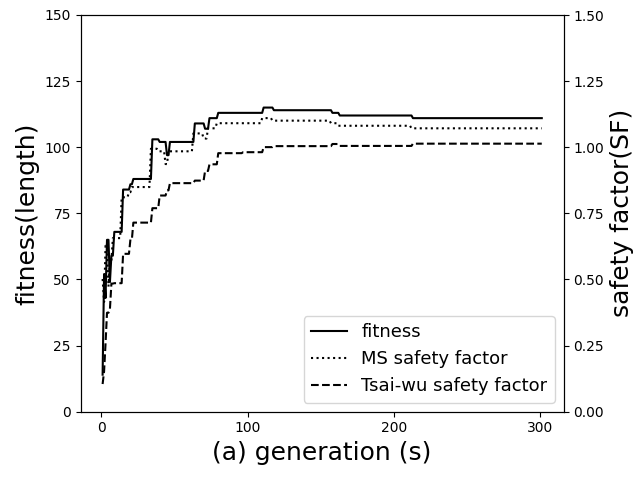
\includegraphics[width=\linewidth]{Figures/chapter4_second_two_distinct_angle_fitness_and_sr.png}
		\end{subfigure}

		\begin{subfigure}[b]{0.8\linewidth}
			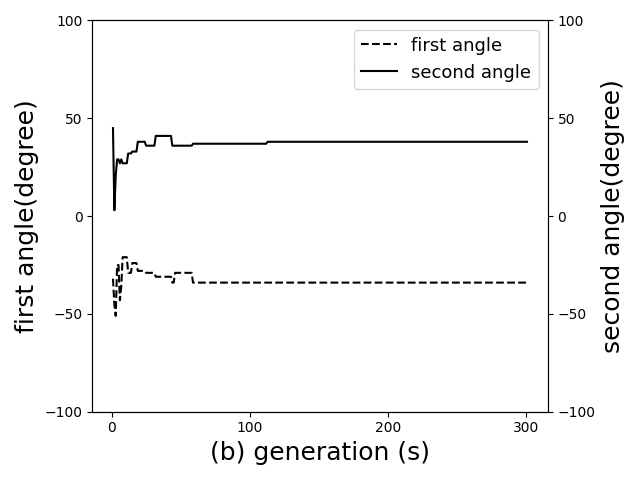
\includegraphics[width=\linewidth]{Figures/chapter4_second_two_distinct_angle_angle_change.png}
		\end{subfigure}

		\begin{subfigure}[b]{0.8\linewidth}
			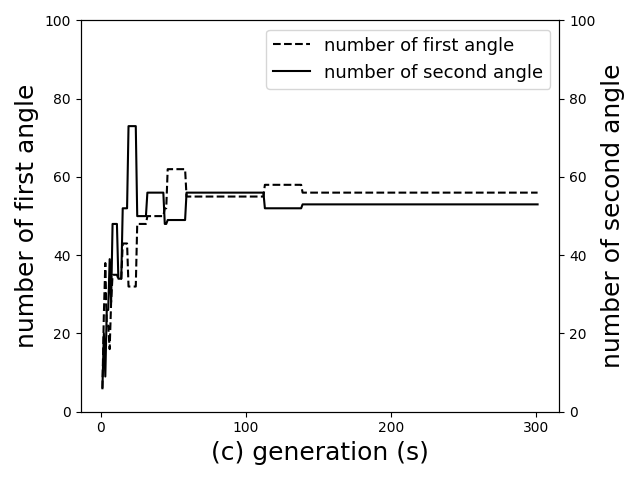
\includegraphics[width=\linewidth]{Figures/chapter4_second_two_distinct_angler_number_change.png}
		\end{subfigure}
	\caption{Two distinct angles}
	\label{fig:two_angles}
\end{figure}
\clearpage
}


Figure \ref{fig:two_angles} (a) shows how the optimal individual's fitness and
strength ratio evolves during the GA process. The solid curve shows the fitness
value, the dashed curve shows the Tsai-wu safety factor, and the dotted curve
shows MS safety factor. If the smaller strength ratio fullfils the constraint,
this laminate must satisfy all the constraints, for simplicity, only the smaller
strength ratio is presented in the figure\ref{fig:three_angles} (a). The method
to chose optimal individual considering two following situations, if no
individual in the current population meets constraint, the one with biggest
fitness is selected as the optimal individual; if there are one or multiple
individuals fullfils requirement, the one with smallest fitness is chosen which
means the smallest one has the biggest priority.  Figure \ref{fig:two_angles}
(b) and \ref{fig:three_angles} (b) show how the every fiber orientation changes , and
Figure \ref{fig:two_angles} (c) and \ref{fig:three_angles} display how the
number of each angles varies.

At the beginning of this GA process, the fitness curves increases very quickly,
becasue individual's two strength ratios are very small, so the difference
between the individual's fitness and the imposed constraint threshold is a big
positive number, so the range of mutaion length is from 0 to $C_l(CT_0 - CV_0 +
CT_1 - CV_1)/2$.  The length of individual increases by n, which is random
number between 0 and $C_l(CT_0 - CV_0 + CT_1 - CV_1)/2$ . As can be seen from
Figure \ref{fig:two_angles} (a), both of optimal individual's fitness and
strength ratio increases very quickly.  The range of angle mutation is from 0 to
$C_a(CT_0 - CV_0 + CT_1 - CV_1)/2$, and the number of each angle also changes
violently. The Figure.\ref{fig:two_angles} (a) and \ref{fig:three_angles} (a) show
this property at the initial stage.  During this stage, increasing individual's length playing a
major role in increasing individual's fitness.

After a couple of generations, the optimal individual's fitness get bigger, and
the difference between individual's fitness and constraint threshold get
smaller. The range of mutation length turn smaller. At
this stage, simply increase the individual's length doesn't make much difference
in improve individual's fitnees, and a better composite laminates lay-up can
dramaticly change the optimal individual's fitness. That's why the fitness curve
oscillated violently in this stage.  At the same time, the strength ratio curve
kept growing smoothly. But the growing speed got more smaller.

When GA comes to its last phase, GA finds individuals that meet all the
constraints.  Now the optimal individual's fitness is greater than the safety
factor. The range of mutation length is from $C_l(CT_0 - CV_0 + CT_1 - CV_1)/2$
to 0. It means individuals need to decrease it's length and improve its internal
structure to meet the constraint. That's why the fitness of optimal individual
kept decreaing, however, the strength ratio curve still is greater then safety
factor.

\afterpage{
\begin{figure}[!htb]
	\centering
		\begin{subfigure}[b]{0.8\linewidth}
			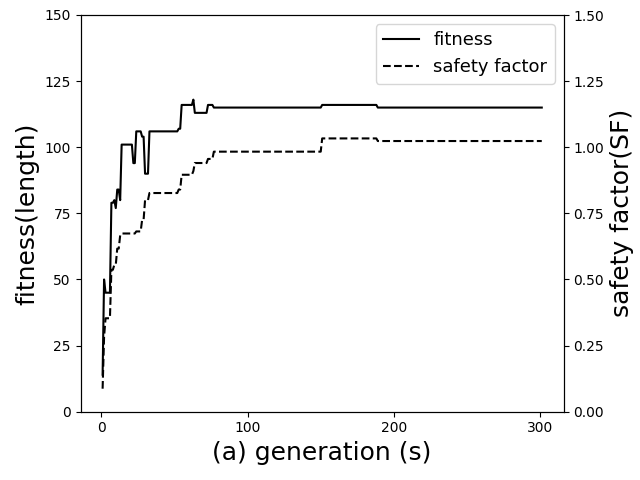
\includegraphics[width=\linewidth]{Figures/chapter4_second_three_distinct_angle_fitness_and_sr.png}
		\end{subfigure}

		\begin{subfigure}[b]{0.8\linewidth}
			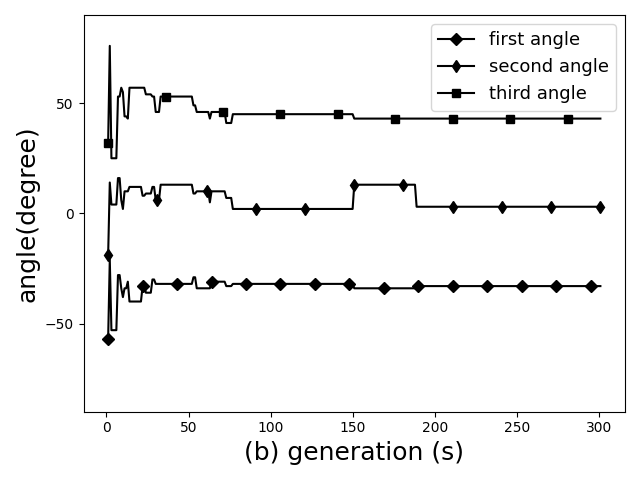
\includegraphics[width=\linewidth]{Figures/chapter4_second_three_distinct_angle_angle_change.png}
		\end{subfigure}

		\begin{subfigure}[b]{0.8\linewidth}
			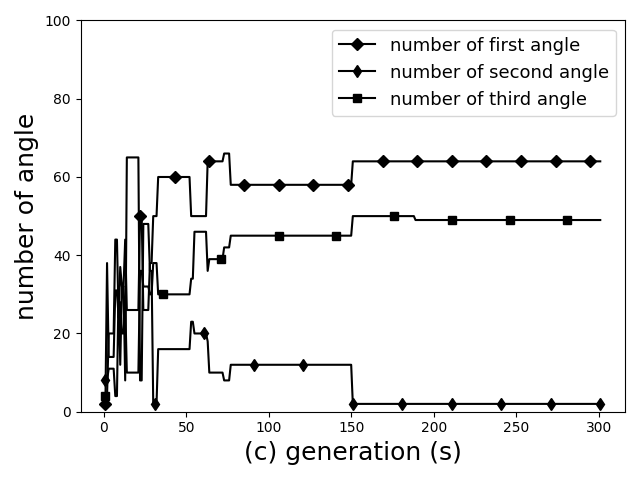
\includegraphics[width=\linewidth]{Figures/chapter4_second_three_distinct_angler_number_of_angle.png}
		\end{subfigure}
	\caption{three distinct angles}
	\label{fig:three_angles}
\end{figure}
\clearpage
}

\begin{table*}
\normalsize
\caption{The optimum lay-ups using three distinct fiber angles under various biaxial loading cases}
\label{T300/5308 material properties}
\centering
\resizebox{13cm}{!}{
\begin{tabular}{clccc}
	\toprule
	\textbf{Loading} $N_{x}/N_{y}/N_{xy}$ \textbf{(MPa m)}   &
	\makecell{\textbf{Optimum lay-up } \\ \textbf{sequences}  }                        &
	\textbf{Laminate thickness} &  \makecell{\textbf{Safety factor } \\
	\textbf{for Tsai-wu}}  &
	\makecell{\textbf{Safety factor } \\ \textbf{for  maximum stress}}
	 \\
	\midrule
	10/5/0                       &  $[37_{27}/\text{-}38_{27}/\text{-}5]_s$            &     110      &  1.0023 & 1.0216\\
	20/5/0                       &  $[34_{24}/\text{-}32_{14}/\text{-}28_{11}]_s$      &     98       &  1.0237 & 1.2089 \\
	40/5/0                       &  $[21_{28}/\text{-}32_{19}/2_3]_s$                  &     100      &  1.0617 & 1.7076\\
	80/5/0                       &  $[\text{-}19_{24}/20_{27}/\text{-}{17}_{16}/\bar{\text{-}17}]_s$  &  109      &  1.0056 & 1.2093 \\
	120/5/0                      &  $[\text{-}19_{33}/12_{13}/16_{28}]_s$              &     148      &  1.0105 &  1.1014\\
	\bottomrule
\end{tabular}
}
\end{table*}


\begin{table*}
	\normalsize
\caption{Comparison with the results of DSA}
\label{tab:comparision}
\centering
\resizebox{13cm}{!}{
\begin{tabular}{c|cccc|lccc}
	\toprule
	\textbf{Loading}	    & \multicolumn {4}{c}{\textbf{Akbulut and Sonmez's\cite{akbulut2008optimum} Study}}   & \multicolumn {4}{c}{\textbf{Present Study}}\\
	\midrule
	 $N_{x}/N_{y}/N_{xy}$   & Optimum lay-up			        & laminate  & TW & MS   & Optimum lay-up & laminate  & TW & MS \\
	  (MPa m)	            & sequences					        & thickness &    &      & sequences	     & thickness &    &    \\
	\midrule
	  10/5/0                 &  $[37_{27}/\text{-}37_{27}]_s$     &  108      &  1.0068  &  1.0277 & $[33_{29}/\text{-}39_{25}/\bar{\text{-}39}]_s$     &     109      &  1.0074      &  1.0246  \\
	  20/5/0                 &  $[31_{23}/\text{-}31_{23}]_s$     &  92       &  1.0208  &  1.1985 & $[33_{22}/\text{-}31_{24}]_s$                      &     92      &  1.0055       &  1.2065    \\
	  40/5/0                 &  $[26_{20}/\text{-}26_{20}]_s$     &  80       &  1.0190  &  1.5381 & $[29_{18}/\text{-}21_{23}/\bar{\text{-}21}]_s$     &     83      &  1.0034       &  1.7350   \\
	  80/5/0                 &  $[21_{25}/\text{-}19_{28}]_s$     &  106      &  1.0113  &  1.2213 & $[\text{-}20_{27}/21_{25}/\bar{25}]_s$             &     105      &  1.0029      &  1.2063    \\
	  120/5/0                &  $[17_{35}/\text{-}17_{35}]_s$     &  140      &  1.0030  &  1.0950 & $[\text{-}18_{34}/17_{36}]_s$                     &     140      &  1.0000      &  1.0898     \\
	\bottomrule
\end{tabular}
}
\end{table*}


Table.\ref{tab:comparision} shows the comparison with the result obtained by
direct search simulated annealing(DSA) algorithm which is proposed by Akbulut
and Sonmez\cite{akbulut2008optimum}.  Both of variant GA and DSA are able to
find feasible solution, but when loading is $N_x=80$, $N_y=5$ MPa m, variant GA
gets a better solution than DSA. In the case that loadings are $N_x=20$, $N_y=5$ MPa m,
and $N_x=120$, $N_y=5$ MPa m,  the proposed GA offers an alternative. Compared
with DSA method, the last advantage of variant GA is the number of layers
doesn't have to be an even number.

\section{Summary}
In this paper, we reviewed the use of variant GA for the optimal design of composite
laminated material under in-plane loading based on Tsai-wu and maximum stress
failure criteria. GA is proposed to search the optimal lay-up for laminated
composite under different loading cases. Two situations are considered under the same
loading, a set of two distinct angles, and three distinct angles. 

By setting the constant values of length mutaion coefficient and angle mutation
coefficient at the beginning, the convergence speed of search process can be
controlled in an explicit way; During the optimization process, GA can adjust
its length mutation range and angle mutation range based on the difference
between individual's constraint values and constraint thresholds.  

Finally, comparison of previous research and current result are presented. In
some cases, the proposed GA in this paper is better off than DSA method.
However, there is still many works to study within this GA, such as the
fine-tuning of parameters taken in this GA.



